This section describes various threats against automatic speaker verification systems, starting from speech synthesis and voice conversion. Previous research on replay attacks and the corresponding countermeasures is presented. In general, all these methods involve generating a spoof signal $s(t)$, based on the target speech signal $x(t)$ of a client, with or without participation of the spoofer voice $y(t)$. The section is concluded with stating motivation and aim of the current research. 

\subsection{Spoofing using speech synthesis}

There is a large variety of speech synthesis algorithms, such as formant, diphone or unit-selection based synthesis. In general, speech synthesis consists in generating intelligible, natural sounding artificial speech for any arbitrary text $c$. The spoofed signal therefore will be generated as:

\begin{equation}
s(t) = g_{x(t)}(c),
\label{eq:tts}
\end{equation}

\noindent where $g_{x(t)}$ denotes text-to-speech mapping using a system with speech units or acoustic models generated based on voice $x(t)$.

State-of-the-art text-to-speech systems use either unit-selection or the hidden Markov model-based synthesis (HTS). Whilst the former requires large amounts of speech data, the latter does not, and can therefore much more easily generate speech targeted towards a specific client. 

Accordingly, in this paper we consider spoofing with HTS synthesis, following the approach described in~\cite{Yamagishi2009}, and using the HMM-based Speech Synthesis System (HTS)\footnote{http://hts.sp.nitech.ac.jp/}. Parametrisation includes STRAIGHT (Speech Transformation and Representation using Adaptive Interpolation of weiGHTed spectrum) features, Mel-cepstrum coefficients and the logarithm of the fundamental frequency (log $F_{0}$) with their delta and acceleration coefficients. Acoustic spectral characteristics and duration probabilities are modelled using multispace distribution hidden semi-Markov models (MSD-HSMM)~\cite{Russell1985}.  Speaker dependent  excitation, spectral and duration models are adapted from corresponding independent models according to a speaker adaptation strategy referred to as constrained structural maximum a posteriori linear regression (CSMAPLR)~\cite{Yamagishi2009a}.  Finally, time domain signals are synthesised using a vocoder based on Mel-logarithmic spectrum approximation (MLSA) filters.  They correspond to STRAIGHT Mel-cepstral coefficients and are driven by a mixed excitation signal and waveforms reconstructed using the pitch synchronous overlap add (PSOLA) method.



\begin{table*}
%\ninept
\begin{center}
    \begin{tabular}{ l | c c c c }
    \hline
     	 Attack & Na\"{i}ve impostor &  Replay & Voice conversion & Speech synthesis\\ 
    \hline
  Speech used & \begin{tabular}{ c } impostor's\\(genuine) \end{tabular} & client's &  \begin{tabular}{ c } impostor's\\(converted) \end{tabular} & synthetic\\
Effort & zero & low & medium-high & high\\
Effectiveness & low &  \textbf{(?)} & medium-high & high\\
 \hline
\hline
    \end{tabular}
    \caption{Comparison of four different attacks in terms of speech used,  required effort and effectiveness.}
		\label{tab::attacks}
   \end{center}
\end{table*}



\subsection{Spoofing by voice conversion}
\label{ssec:vconv}

Voice conversion has been used to spoof speaker verification systems since the late 90s~\cite{Pellom1999},~\cite{Perrot2005}. When comparing the replay threat with that of voice conversion, we used the approach to voice conversion originally presented in~\cite{Matrouf2005}. Here, the spoofing signal $s(t)$ (or $S(f)$ in the spectral domain) is generated by filtering at the frame level the speech signal of a spoofer $y(t)$ in the spectral domain as follows:

\begin{equation}
S(f) = \frac{\left|H_{x}(f)\right|}{\left|H_{y}(f)\right|}Y(f)
\label{eq:conversioneq}
\end{equation}

\noindent where $H_{x}(f)$ and $H_{y}(f)$ are the vocal tract transfer functions of the targeted speaker and the spoofer respectively.  $Y(f)$ is the spoofer's speech signal in the spectral domain whereas $S(f)$ denotes the result after voice conversion.  As such, $y(t)$ is mapped or converted towards the target in a spectral-envelope sense, which is sufficient to overcome most ASV systems. 

$H_x(f)$ is determined from a set of two Gaussian mixture models (GMMs).  The first, denoted as the automatic speaker recognition (asr) model in the original work, is related to ASV feature space and utilised for the calculation of a posteriori probabilities whereas the second, denoted as the filtering (fil) model, is a tied model of linear predictive cepstral coding (LPCC) coefficients from which $H_x(f)$ is derived.  LPCC filter parameters are obtained according to:

\begin{equation}
x_{fil} = \sum\limits_{i=1}^{M}p(g_{asr}^{i}|y_{asr}) \mu_{fil}^{i}
\label{eq:EMit}
\end{equation}

\noindent where $p(g_{asr}^{i}|y_{asr})$ is the a posteriori probability of Gaussian component $g_{asr}^{i}$ given the frame $y_{asr}$ and $\mu_{fil}^{i}$ is the mean of component $g_{fil}^{i}$ which is tied to $g_{asr}^{i}$.  $H_{x}(f)$ is estimated from $x_{fil}$ using an LPCC-to-LPC transformation and a time-domain signal is synthesised from converted frames with a standard overlap-add technique. Full details can be found in~\cite{Bonastre2007,Matrouf2005,Bonastre2006}.


\subsection{Spoofing by replay}

Replay attacks are an example of low-effort spoofing; they require simply the replaying of a previously captured speech signal.  
In the absence of suitable countermeasures and considering the widespread availability of consumer devices with reasonable quality sound systems, replay attacks can typically be realised with ease.  
%The risk of playback attacks is even higher if recordings of a speaker are publicly available and is
Furthermore, they are pertinent in the case of both text-dependent and text-independent systems through the cutting and pasting of short speech intervals.  
Paradoxically, given that they have potential to attenuate channel effects which might be introduced through recording and replaying, channel-compensation and other techniques which aim to attenuate intersession variability have potential to work in favour of the replay attacker.
Since almost all state-of-the-art speaker verification systems include some form of intersession compensation, then one must consider most systems at least somewhat vulnerable. 
All of these factors point towards the significant threat of replay attacks and the importance of developing suitable anti-spoofing countermeasures.

Generally, in replay attack the spoofed signal can be represented as:
\begin{equation}
s(t) = x(t)*h(t),
\label{eq:replay}
\end{equation}

\noindent where * denotes convolution and $h(t)$ denotes the impulse response of replay hardware and replay environment. When modelling $h(t)$, the impact of the following elements is usually considered:

\begin{itemize}
\item acoustic effects introduced by the recording device;
\item acoustic conditions in the environment where the voice was acquired;
\item acoustic effects of the replay device, and the
\item acoustic conditions in the environment where the attack takes place. 
\end{itemize}

\begin{figure}
	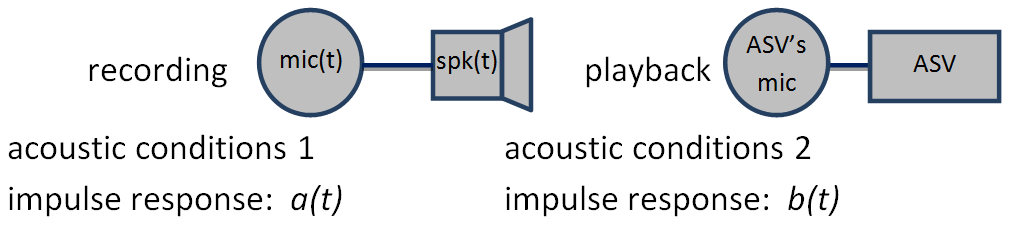
\includegraphics[width=1\linewidth]{Figs/replay.png}

	\caption{Schematic diagram of replay.}
	\label{fig::Replay}
\end{figure}


Therefore, the spoofing signal $s(t)$ in case of playback can be represented by:

\begin{equation}
s(t) = x(t)* mic(t) * a(t) * spk(t) * b(t)
\label{eq::playback}
\end{equation}

where * denotes convolution, $mic(t)$ and $spk(t)$ are impulse responses of the microphone and the speaker, respectively, and $a(t)$ and $b(t)$ are impulse responses of recording and replay environments, respectively (see Fig.~\ref{fig::Replay}). 

While a great deal of attention has been paid to medium- and high-effort spoofing attacks (reviews can be found in~\cite{handbookChapter,Wu2014a}), only few studies have addressed replay.  
The work in~\cite{Lindberg1999} assessed the vulnerabilities of an HMM-based, text-dependent ASV system with concatenated digits.  
While results showed that replay attacks are highly effective, experiments were conducted with data collected from only two speakers.
The work in~\cite{Villalba2010} investigated replay using recordings which were collected with close-talk or far-field microphones and then replayed over an analogue or digital telephony channel. 
The work was conducted with a similarly small corpus with five speakers and showed that a joint factor analysis (JFA) ASV system was vulnerable to replay attacks -- the FAR at the EER threshold increased from 1\% to almost 70\%. The authors in~\cite{Wu2014} investigated a text-dependent ASV system exposed to speech played back from a laptop. Using the RSR2015 corpus the authors showed that the EER increased from around 4\% to more than 20\%.


% COMMENT: note that I removd the following.  I don't find that is really necessary for the other material in this section and it will help to differentiate more from the BIOSIG paper if we move this material to the section which relates to your contribution rather than the past work.





\subsection{Comparison of spoofing attacks}
\label{sec::algorithms::comparison}


Table~\ref{tab::attacks} contrasts na\"{i}ve (zero-effort) impostor accesses and spoofing attacks: replay, voice conversion and speech synthesis.  
They are ordered in terms of the effort or skill needed to implement each attack successfully~\cite{Wu2014a}. 
Replay attacks require slightly increased effort compared to na\"{i}ve imposture (need for recording and replay hardware). 
Voice conversion and speech synthesis require specialised algorithms, in addition to recording hardware to collect, analyse and parametrise the target voice. 
They belong to a class of higher-effort spoofing attacks. 
While voice conversion is still based upon the conversion of an original speech signal, speech synthesis starts with text input. 
Its conversion to a convincing speech signal indicative of a particular speaker requires the most effort of all three attacks.

One may reasonably suppose that the effectiveness of each attack is linked to the effort involved; the higher the effort, the greater the impact on ASV performance. 
However, the results of preliminary experiments described in~\cite{Alegre2014} found the contrary, showing that replay attacks pose high risk, being effective in overcoming an ASV system while being the easiest to implement, hence the motivation of this work. In contrast to~\cite{Alegre2014}, in this work we will consider nine different playback setups (instead of just one) and we will verify the effectiveness of two countermeasures against replay.
%can be theis in fact very high, taking into account low-effort required to undertake the attack. This observation will be further verified in this work.
